%Copyright (c) 2020 Paul Stahr

%Permission is hereby granted, free of charge, to any person obtaining a copy
%of this software and associated documentation files (the "Software"), to deal
%in the Software without restriction, including without limitation the rights
%to use, copy, modify, merge, publish, distribute, sublicense, and/or sell
%copies of the Software, and to permit persons to whom the Software is
%furnished to do so, subject to the following conditions:

%The above copyright notice and this permission notice shall be included in all
%copies or substantial portions of the Software.

%THE SOFTWARE IS PROVIDED "AS IS", WITHOUT WARRANTY OF ANY KIND, EXPRESS OR
%IMPLIED, INCLUDING BUT NOT LIMITED TO THE WARRANTIES OF MERCHANTABILITY,
%FITNESS FOR A PARTICULAR PURPOSE AND NONINFRINGEMENT. IN NO EVENT SHALL THE
%AUTHORS OR COPYRIGHT HOLDERS BE LIABLE FOR ANY CLAIM, DAMAGES OR OTHER
%LIABILITY, WHETHER IN AN ACTION OF CONTRACT, TORT OR OTHERWISE, ARISING FROM,
%OUT OF OR IN CONNECTION WITH THE SOFTWARE OR THE USE OR OTHER DEALINGS IN THE
%SOFTWARE.

\documentclass[11pt, a4paper, UKenglish, parskip=half+, oneside]{scrbook}
\usepackage{verbatim}
\usepackage{float}
\usepackage{wrapfig}
\usepackage{xcolor}
\usepackage{listings}
\newcommand{\slots}{slots}
\renewcommand{\bf}{\textbf}
\usepackage[siunitx]{circuitikz}
\usepackage{tikz}
\usetikzlibrary{fit}
\usetikzlibrary{er,positioning}
	\author{Paul Stahr}
	\title{Lapcounter with Raspberry pi}

\lstset{backgroundcolor=\color{lightgray!60},
  frame=trbl,
  rulecolor=\color{black!30},
  xrightmargin=7pt}

\begin{document}
\maketitle
\chapter{Introduction}
This is a testimonial for building a lapcounter for slotcars with the rasperry pi. It contains a guide how to wire the necessary hardware and also a program to cover the main functionality. Any feedback and improvement suggestions are very welcome.
\chapter{Hardware}
In my setup I used a raspberry pi 3, but I won't expect any problems using other versions.\\
For checking if cars crossed the starting line it turned out to be most reliable to have fototransistors in the track and some leds above. Another promising attempt to use the slot itself turned out to miss the car occasionally as they hopped over the barrier from time to time. To have a compact device I used the 7" Touchscreen Display which could be directly connected.
\section{Components}
\begin{table}[H]
\begin{tabular}{l l l l}
Item& Amount & Article number & Price\\\hline
Raspberry PI 4 B 2 GB All-In-Bundle & 1 &RPI 4B 2GB ALLIN &66,50 \\
7" Touchscreen Display & 1 & RASPBERRY PI 7TD&64,50\\
NE 555 DIP & \slots &NE 555 DIP& 0.17 \\
Resistor 470$\Omega$ & \slots&K-O RD12JN471T52&0.08 \\
Resistor 10k & \slots& K-O RD12JN103T52 & 0.08\\
Resistor 100k & \slots& K-O RD12JN104T52& 0.08 \\
Led V 510 Flat Led Rot& \slots &V 510& 0.10 \\
Phototransistor BPW 42 & \slots& BPW 42& 0.29\\
LED 3MM GN LED & 1& LED 3MM GN& 0.07\\
Bluetooth keyboard& & (1) \\
MT3608 & 1& & 3.29\\
\end{tabular}
\caption{Table of components}
\end{table}

\ctikzset{bipoles/length=1cm} % Controls bipoles scale
\section{Wiring}
\begin{wrapfigure}{r}{0.7\textwidth}
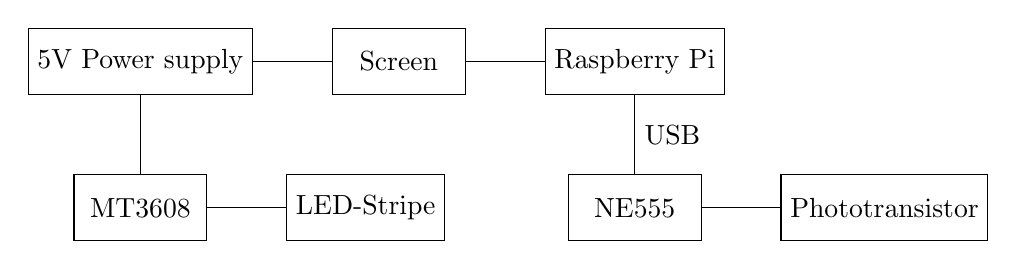
\begin{tikzpicture}[auto,node distance=1cm]
\node[entity] (screen) {Screen}
[grow=up,sibling distance=2cm];
%child {node[attribute] {Attribute 2}};
% Now place a relation (ID=rel1)
%\node[relationship] (rel1) [below right = of screen] {Relation 1};
% Now the 2nd entity (ID=rel2)
\node[entity] (rpi) [right = of screen]	{Raspberry Pi};
\node[entity] (ne) [below = of rpi]	{NE555};
\node[entity] (ph) [right = of ne]	{Phototransistor};
\node[entity] (power) [left = of screen]	{5V Power supply};
\node[entity] (mt) [below = of power]	{MT3608};
\node[entity] (led) [right = of mt]	{LED-Stripe};
\path (screen) edge (rpi);
\path (power) edge	(screen);
\path (power) edge	(mt);
\path (mt) edge	(led);
\path (rpi) edge node {USB} (ne);
\path (ne) edge	(ph);
\end{tikzpicture}
\caption{High level connection Diagram}
\end{wrapfigure}
\begin{wrapfigure}{r}{0.4\textwidth}
	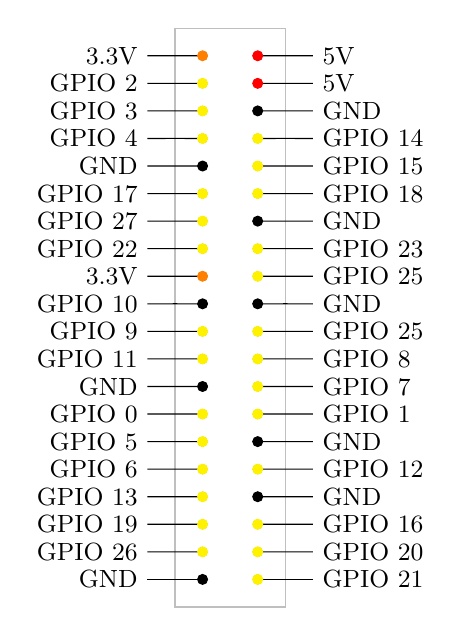
\begin{tikzpicture}[scale=0.7]
	\draw[color=lightgray] (0.5,-0.5) rectangle (2.5,10);
	\foreach \j/\namea/\cola/\nameb/\colb in {
		0/3.3V/orange/5V/red,
		1/GPIO 2/yellow/5V/red,
		2/GPIO 3/yellow/GND/black,
		3/GPIO 4/yellow/GPIO 14/yellow,
		4/GND/black/GPIO 15/yellow,
		5/GPIO 17/yellow/GPIO 18/yellow,
		6/GPIO 27/yellow/GND/black,
		7/GPIO 22/yellow/GPIO 23/yellow,
		8/3.3V/orange/GPIO 25/yellow,
		9/GPIO 10/black/GND/black,
		10/GPIO 9/yellow/GPIO 25/yellow,
		11/GPIO 11/yellow/GPIO 8/yellow,
		12/GND/black/GPIO 7/yellow,
		13/GPIO 0/yellow/GPIO 1/yellow,
		14/GPIO 5/yellow/GND/black,
		15/GPIO 6/yellow/GPIO 12/yellow,
		16/GPIO 13/yellow/GND/black,
		17/GPIO 19/yellow/GPIO 16/yellow,
		18/GPIO 26/yellow/GPIO 20/yellow,
		19/GND/black/GPIO 21/yellow}
	{
		\draw (1,9.5-\j/2) to [short,o-] (0,9.5-\j/2){} node[left]{\small \namea};
		\draw (2,9.5-\j/2) to [short,o-] (3,9.5-\j/2){} node[right]{\small \nameb};
		\fill[fill=\cola] (1,9.5-\j/2) circle(0.1);
		\fill[fill=\colb] (2,9.5-\j/2) circle(0.1);
	}
	\end{tikzpicture}
\caption{Raspberry pi pinlayout}	
\end{wrapfigure}
To connect the display power, the illumination and the senors we will use the gpio of the raspberry pi. For the connection from the photodiode to the input-circuit I uses usb-connectors. I put the \ref{timercirquit} between the photodiode and the input of the raspberry pi, which pulls down the voltage for a defined amount of time whenever a car crosses.
\subsection{GPIO}
The gpio of the raspberry pi provides low level commiunication with electric circuits. Here is a complete diagram of all connectors. Please notice that the 3.3V are provided by the integrated voltage regulator and only allow very small loads.

\begin{wrapfigure}{r}{0.7\textwidth}
\label{timercirquit}
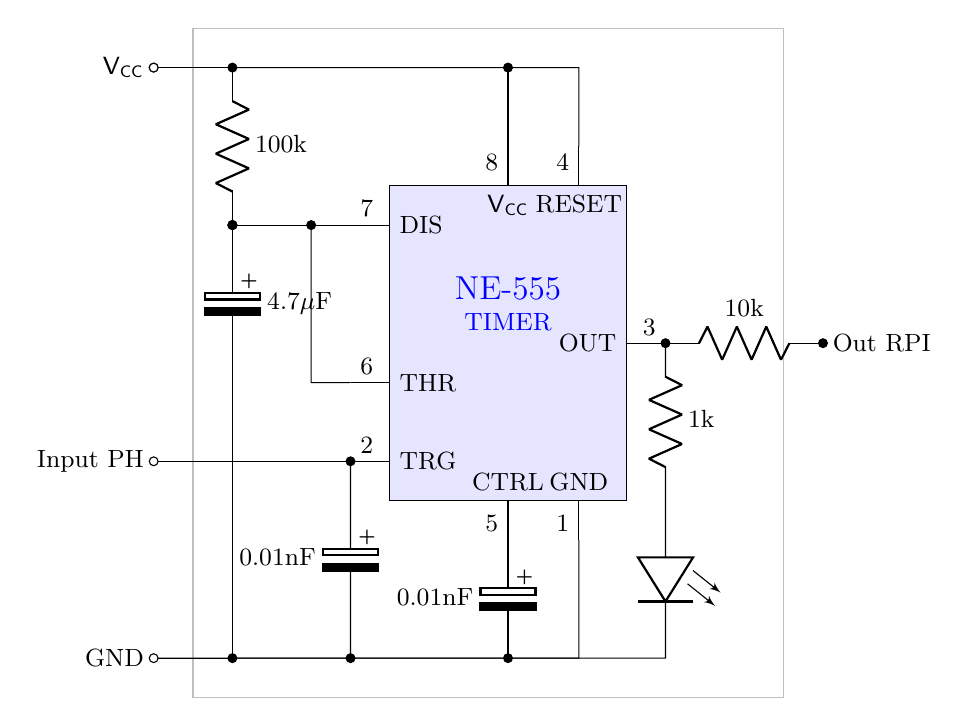
\begin{tikzpicture}[font=\small]

\begin{scope}
\def\TIMER555(#1)#2{%
	\begin{scope}[shift={(#1)}]
	\draw[fill=blue!10] (-1.5,-2) rectangle (1.5,2); % The body of IC
	% Label and component identifier.
	\draw[blue] (0,0.5) node [align=center]{\large NE-555\\TIMER}; % IC LABEL
	\draw (0.9,-2) node [above]{GND} -- +(0,-0.5) node [anchor=-45]{1} coordinate (#2 GND); % Pin 1 GND
	\draw (-1.5,-1.5) node [right]{TRG} -- +(-0.5,0) node [anchor=-135]{2} coordinate (#2 TRG); % Pin 2 TRG
	\draw (1.5,0) node [left]{OUT} -- +(0.5,0) node [anchor=-45]{3} coordinate (#2 OUT); % Pin 3 OUT  
	\draw (0.9,2) node [below]{RESET} -- +(0,0.5) node [anchor=45]{4} coordinate (#2 RESET); % Pin 4 RESET
	\draw (0,-2) node [above]{CTRL} -- +(0,-0.5) node [anchor=-45]{5} coordinate (#2 CTRL); % Pin 5 CTRL
	\draw (-1.5,-.5) node [right]{THR} -- +(-0.5,0) node [anchor=-135]{6} coordinate (#2 THR); % Pin 6 THR
	\draw (-1.5,1.5) node [right]{DIS} -- +(-0.5,0) node [anchor=-135]{7} coordinate (#2 DIS); % Pin 7 DIS
	\draw (0,2) node [below]{$\mathsf{V_{CC}}$} -- +(0,0.5) node [anchor=45]{8} coordinate (#2 VCC); % Pin 8 VCC
	\end{scope}
}

\draw[color=lightgray] (-4,-4.5) rectangle (3.5,4.0);
\TIMER555(0,0){1}

%Place polarization nodes:
\draw (-4.5,3.5) node[ocirc] (VCC){} node[left]{$\mathsf{V_{CC}}$};
\draw (-4.5,-4) node[ocirc] (GND){} node[left]{GND};
\draw (-4.5,-1.5) node[ocirc] (INPUT){} node[left]{Input PH};
\draw(VCC) % Start point
to [short, o-] ++(1,0) coordinate (NOD1) % Use auxiliar coordinate (NOD1)
to [R, l^=100k,*-*] (1 DIS -| NOD1) % to the point in the intersection between NOD1 and 1 DIS
to [eC,l^=$4.7\mu$F,*-] ++(0,-2)
to [short,-*] (GND -| NOD1)
to [short] (GND);

\draw(1 VCC) to [short, -*] (1 VCC |- NOD1);
\draw(1 RESET) to [short] (1 RESET |- NOD1) to [short] (NOD1);
\draw(1 DIS) to [short, -*] (1 DIS -| NOD1);
\draw(1 THR) to [short] ++ (-0.5,0) coordinate (NOD2) to [short,-*] (1 DIS -| NOD2);
\draw(1 CTRL) to [eC,l_=0.01nF, -*] (1 CTRL |- GND);
\draw(1 GND) to [short] (1 GND |- GND) to [short] (GND -| NOD1);
\draw(INPUT) to [short, -] (INPUT -| NOD1);
\draw(1 TRG) to [short, *-] (INPUT -| NOD1);



%Place input/output nodes
%\draw[color=blue,line width=2] (1 TRG) to [short] ++(-0.55,0) node[ocirc] (TRG){} node[below]{Trigger};
%\draw(1 TRG) to [short] ++(-2,0) (TRG){};
\draw(1 TRG) to [eC,l_=0.01nF, -*] (1 TRG |- GND);
\draw (1 OUT) to [R, l^=$10$k, -*] ++ (2,0) node[right]{Out RPI};
\draw (1 OUT) to [R,l^=1k, *-] ++ (0,-2) to [empty led] (1 OUT |- GND) to (GND);
%\draw[color=red,line width=2] (1 OUT) to [short] ++(0.55,0) node[ocirc](OUT){} node[below]{Out};
\end{scope}
\end{tikzpicture}
\caption{Delay circuit}
\end{wrapfigure}
\subsection{NE-555}
The timer NE-555 is maybe the most often produced integrated circuit in history. It allows us to work as a delay, extending the signal of a led covered for a short amount of time to trigger a signal which lasts over a second. As the raspberry pi supports interrupts it should be possible to directly connect the phototransistor to its gpio input.
\begin{wrapfigure}{r}{0.2\textwidth}
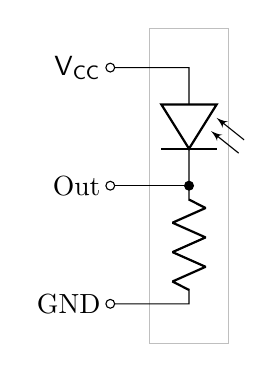
\begin{tikzpicture}
\begin{scope}[shift={(-7,0)}]
\draw[color=lightgray] (0.5,-0.5) rectangle (1.5,3.5);
\draw (0,0) node[ocirc] (GND){} node[left]{GND};
\draw (0,3) node[ocirc] (VCC){} node[left]{$\mathsf{V_{CC}}$};
\draw (0,1.5) node[ocirc] (OUT){} node[left]{Out};
\draw(VCC) to [short] ++ (1,0) to [empty photodiode] ++ (0,-1.5) to [R] ++(0,-1.5) to [short] (GND);
\draw (OUT) to [short, -*] ++ (1,0);
\end{scope}
\end{tikzpicture}
\caption{Photodiode}
\end{wrapfigure}
\subsection{Connectors}
As you have to put the phototransistors into the racetrack you might not want to have fixed cables running all the way up to the GPIO of the Raspberry pi. You can use any connector you like, but I found usb very handy because this allowed me to just solder Type-A and Mini-A connectors on all boards and use ordinary cables for the connections in between. I tried to keep as close to the original standart as possible by using the outer lanes for power supply and the inner one for data transmition.
\begin{wrapfigure}{r}{0.6\textwidth}
	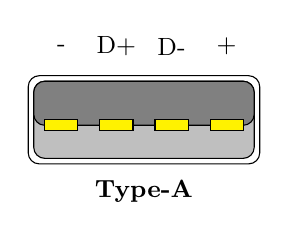
\begin{tikzpicture}[scale=0.7]
	\filldraw[fill=white, draw=black, rounded corners] (-2.1,0.1) rectangle (2.1,-1.5);
	\filldraw[fill=lightgray, draw=black, rounded corners] (-2.0,0) rectangle (2.0,-1.4);
	\filldraw[fill=gray, draw=black, rounded corners] (-2,0) rectangle (2,-0.8);
	\foreach \i/\t in {-1.5/-,-0.5/D+,0.5/D-,1.5/+}
	{
		\filldraw[fill=yellow, draw=black] (\i-0.3,-.7) rectangle node[yshift=1.0cm]{\small \t} (\i+0.3,-0.9) ;
	}
	\node at (0,-2) {\small \textbf{Type-A}};
	\end{tikzpicture}
	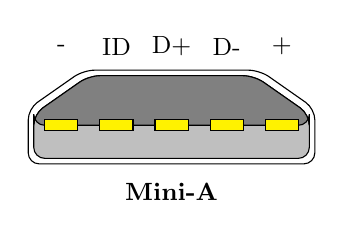
\begin{tikzpicture}[scale=0.7]
	\fill[fill=white, draw=black,rounded corners] 
	(-1.6,0.2) -- (1.6,0.2) -- (2.6,-0.5) -- (2.6,-1.5) -- (-2.6,-1.5) -- (-2.6,-0.5) -- cycle;
	\fill[fill=lightgray, draw=black,rounded corners] 
	(-1.5,0.1) -- (1.5,0.1) -- (2.5,-0.6) -- (2.5,-1.4) -- (-2.5,-1.4) -- (-2.5,-0.6) -- cycle;
	\fill[fill=gray, draw=black,rounded corners] 
	(-1.5,0.1) -- (1.5,0.1) -- (2.5,-0.6) -- (2.5,-0.8) -- (-2.5,-0.8) -- (-2.5,-0.6) -- cycle;
	\foreach \i/\t in {-2/-,-1/ID,0/D+,1/D-,2/+}
	{
		\filldraw[fill=yellow, draw=black] (\i-0.3,-.7) rectangle node[yshift=1.0cm]{\small \t} (\i+0.3,-0.9) ;
	}
	\node at (0,-2) {\small\textbf{Mini-A}};
	\end{tikzpicture}
	\caption{USB-Pins}
\end{wrapfigure}
\subsection{Illumination}
For illumination it was conventient to use led-stripe. The general problem here is, that most of them work with 12V. Also you might want to have an adjustable brightness. For these kind of tasks a MT3608 Step Up converter is a cheap and handy solution. Just connect it to the 5V supply and the led-stripe to its output.
\begin{wrapfigure}{r}{0.6\textwidth}
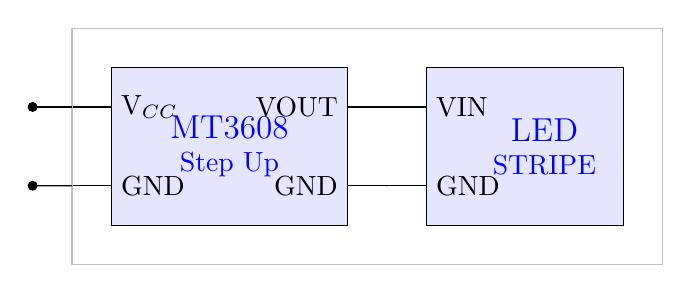
\begin{tikzpicture}
\begin{scope}[shift={(-2,6.5)}]

\def\MT3608(#1)#2{%
	\begin{scope}[shift={(#1)}]
	\draw[fill=blue!10] (-1.5,-1.5) rectangle (1.5,0.5); % The body of IC
	%	\draw[blue] (2,2.5) node []{\large \bf U - #2}; % IC LABEL
	\draw[blue] (0,-0.5) node [align=center]{\large MT3608\\Step Up}; % IC LABEL
	\draw (-1.5,-1) node [right]{GND} -- +(-0.5,0) node [anchor=-135]{} coordinate (#2 GND); % Pin 2 TRG
	\draw (1.5,0) node [left]{VOUT} -- +(0.5,0) node [anchor=-45]{} coordinate (#2 VOUT); % Pin 3 OUT  
	\draw (1.5,-1) node [left]{GND} -- +(0.5,0) node [anchor=-45]{} coordinate (#2 GNDD); % Pin 3 OUT  
	\draw (-1.5,0) node [right]{V$_{CC}$} -- +(-0.5,0) node [anchor=-135]{} coordinate (#2 VIN); % Pin 7 DIS
	\end{scope}
}

\def\LEDSTRIPE(#1)#2{%
	\begin{scope}[shift={(#1)}]
	\draw[fill=blue!10] (-1.5,-1.5) rectangle (1,0.5); % The body of IC
	%	\draw[blue] (2,2.5) node []{\large \bf U - #2}; % IC LABEL
	\draw[blue] (0,-0.5) node [align=center]{\large LED\\STRIPE}; % IC LABEL
	\draw (-1.5,-1) node [right]{GND} -- +(-0.5,0) node [anchor=-135]{} coordinate (#2 GND); % Pin 2 TRG
	\draw (-1.5,0) node [right]{VIN} -- +(-0.5,0) node [anchor=-135]{} coordinate (#2 VIN); % Pin 7 DIS
	\end{scope}
}
\MT3608(0,0){1} 
\LEDSTRIPE(4,0){2} 
\draw[color=lightgray] (-2,-2) rectangle (5.5,1);
\draw(1 VIN) to [short, -*] ++(-0.5,0);
\draw(1 GND) to [short, -*] ++(-0.5,0);
\draw(1 VOUT) to [short, -] (2 VIN);
\draw(1 GNDD) to [short, -] (2 GND);
\end{scope}
\end{tikzpicture}
\caption{Power supply for Led-stripe}
\end{wrapfigure}
\begin{comment}



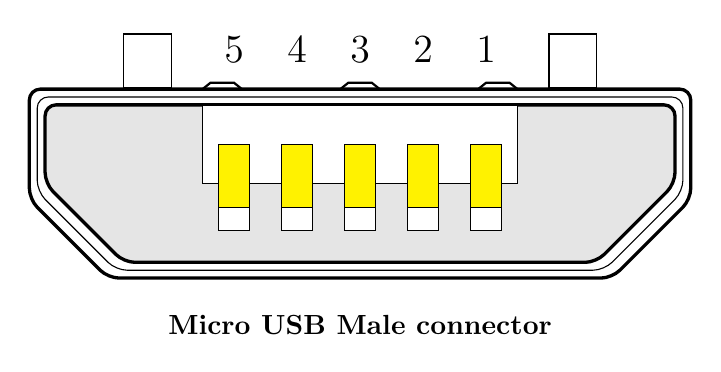
\begin{tikzpicture}

\draw[very thick,rounded corners] 
(-.2,.2) -- (8.2,0.2) -- (8.2,-1.2) -- (7.2,-2.2) -- (0.8,-2.2) -- (-.2,-1.2) -- cycle;
\draw[thin,rounded corners] 
(-.1,.1) -- (8.1,0.1) -- (8.1,-1.1) -- (7.1,-2.1) -- (0.9,-2.1) -- (-.1,-1.1) -- cycle;
\fill[gray!20, draw=black, very thick,rounded corners] 
(0,0) -- (8,0) -- (8,-1) -- (7,-2) -- (1,-2) -- (0,-1) -- cycle;

\draw[thick] (2,.2) -- ( 2.1,.28) -- (2.4,.28) -- (2.5,.2);
\draw[thick] (3.75,.2) -- ( 3.85,.28) -- (4.15,.28) -- (4.25,.2);
\draw[thick] (6,.2) -- ( 5.9,.28) -- (5.6,.28) -- (5.5,.2);

\filldraw[fill=white, draw=black] (2,-.01) rectangle (6,-1);
\filldraw[fill=white, draw=black] (1,.9)   rectangle (1.6,0.22);
\filldraw[fill=white, draw=black] (6.4,.9) rectangle (7,0.22);
\filldraw[fill=yellow, draw=black] (2.2,-.5) rectangle node[yshift=1.6cm]{\Large 5} (2.6,-1.3) ;
\filldraw[fill=white, draw=black]  (2.2,-1.3) rectangle (2.6,-1.6);
\filldraw[fill=yellow, draw=black] (3.0,-.5) rectangle node[yshift=1.6cm]{\Large 4} (3.4,-1.3);
\filldraw[fill=white, draw=black]  (3.0,-1.3) rectangle (3.4,-1.6);
\filldraw[fill=yellow, draw=black] (3.8,-.5) rectangle node[yshift=1.6cm]{\Large 3} (4.2,-1.3);
\filldraw[fill=white, draw=black]  (3.8,-1.3) rectangle (4.2,-1.6);
\filldraw[fill=yellow, draw=black] (4.6,-.5) rectangle node[yshift=1.6cm]{\Large 2}(5.0,-1.3);
\filldraw[fill=white, draw=black]  (4.6,-1.3) rectangle (5.0,-1.6);
\filldraw[fill=yellow, draw=black] (5.4,-.5) rectangle node[yshift=1.6cm]{\Large 1} (5.8,-1.3);
\filldraw[fill=white, draw=black]  (5.4,-1.3) rectangle (5.8,-1.6);
\node at (4,-2.8) {\textbf{Micro USB Male connector}};
%\node at (2.2, .8) {\textbf{5}}; \node at (3, .8) {\textbf{4}}; \node at (3.8, .8) {\textbf{3}}; \node at (4.6, .8) {\textbf{2}}; \node at (5.4, .8) {\textbf{1}};
\end{tikzpicture}
\end{comment}

\begin{comment}
	
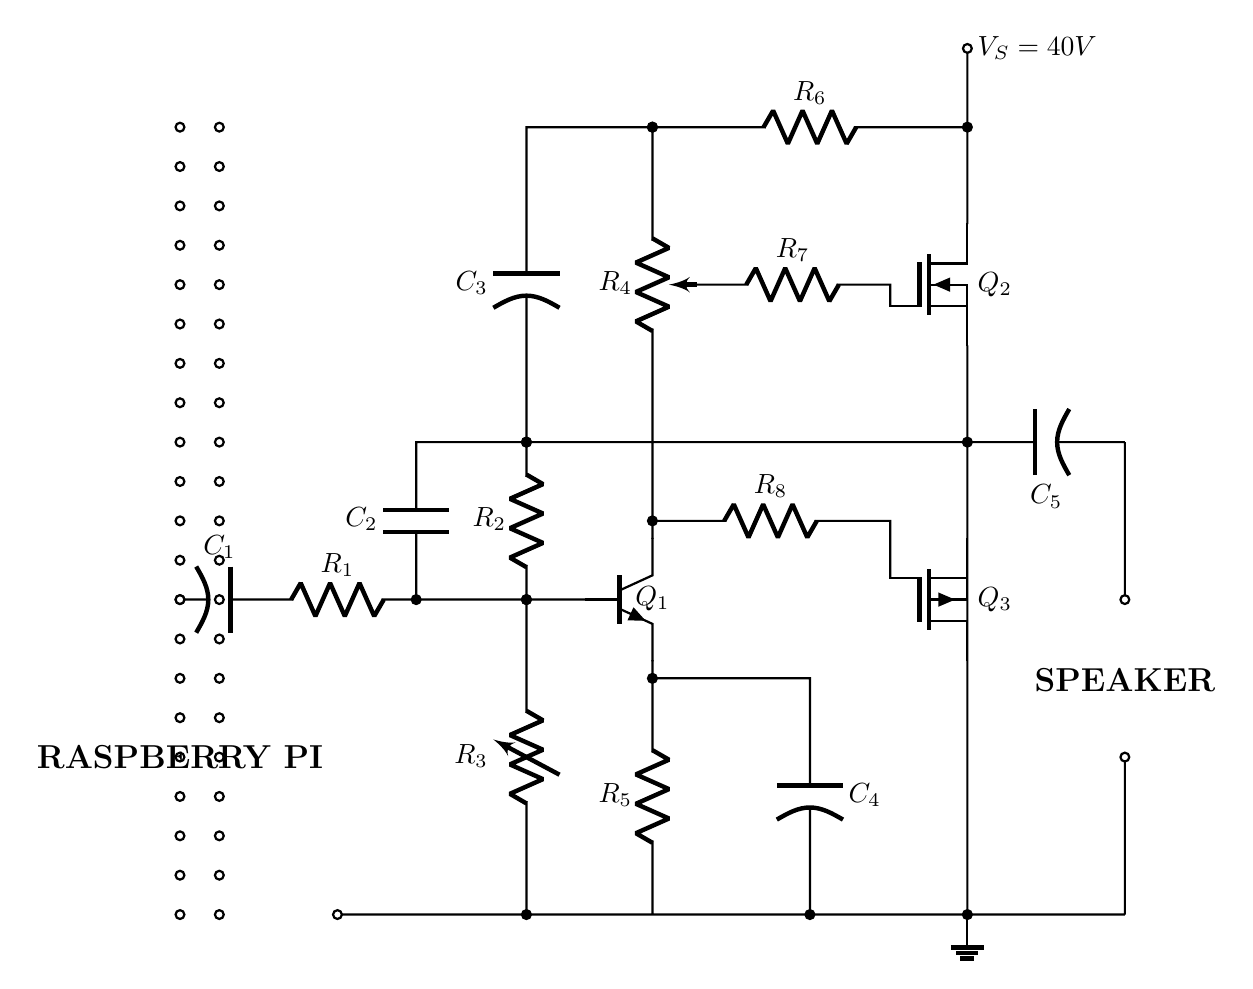
\begin{tikzpicture}[scale=2]
  \draw[color=black, thick]
  \foreach \i in {0,...,1}
  {
  	\foreach \j in {0,...,20}
  	{
  		(\i/4,\j/4) to [short,o-] (\i/4,\j/4){}
  	}
  }
  
    (1,0) to [short,o-] (6,0){} % Baseline for connection to ground
    % Input and ground
    (0,1) node[]{\large{\textbf{RASPBERRY PI}}}
    % Connection of passive components
    (5,0) node[ground]{} node[circ](4.5,0){}
    (0,2) to [pC, l=$C_1$, o-] (0.5,2)
    to [R,l=$R_1$,](1.5,2)
    to node[short]{}(2.6,2)
    (1.5,2) to [C, l=$C_2$, *-] (1.5,3) -| (5,3)
    (2.2,2) to [R, l=$R_2$, *-*] (2.2,3)
    (2.2,3) to [pC, l=$C_3$, *-] (2.2,5) -| (3,5)
    % Transistor Bipolar Q1
    (3,0) to [R,l=$R_5$,-*] (3,1.5)
    to [Tnpn,n=npn1] (3,2.5)
    (npn1.E) node[right=3mm, above=5mm]{$Q_1$} % Labelling the NPN transistor
    (4,0) to [pC, l_=$C_4$, *-] (4, 1.5)--(3,1.5)
    (2.2,0) to [vR, l=$R_3$, *-*] (2.2,2)
    (3,2.5) to node[short]{}(3,3)
    (3,5) to [pR, n=pot1, l_=$R_4$, *-] (3,3)
    (3,5) to [R, l=$R_6$, *-] (5,5)
    to [short,*-o](5,5.5) node[right]{$V_S=40 V$}
    % Mosfet Transistors
    (5,3) to [Tnigfetd,n=mos1] (5,5)
    (mos1.B) node[anchor=west]{$Q_2$} % Labelling MOSFET Q2 Transistor
    (pot1.wiper)  to [R, l=$R_7$] (4.5,4) -| (mos1.G)
    (5,1.5) to [Tpigfetd,n=mos2] (5,2.5)
    (5,0) to (mos2.S)
    (3,2.5) to [R, l=$R_8$, *-] (4.5,2.5)
    -| (mos2.G)
    (mos2.B) node[anchor=west]{$Q_3$} % Labelling MOSFET Q3 Transistor
    % Output
    (6,3) to [pC, l=$C_5$,-*](5,3)
    (6,3) to [short,-o] (6,2){}
    (mos1.S)--(mos2.D)
    (6,0) to [short,-o] (6,1){} node[above=7mm]{\large{\textbf{SPEAKER}}}
    ;
\end{tikzpicture}
\end{comment}
\chapter{Software}
\section{Compiling}
The program uses Allegro to show the results. In theory it should be possible to use it on any machine, which supports linux and opengl, I tested it on a x86 platform and on the raspberry pi. If you are using debian, please install the following packages:
\begin{lstlisting}[language=bash,caption={Required packages},breaklines=true]
sudo aptitude install build-essential g++ liballegro5-dev freeglut3-dev libboost-thread-dev libboost-system-dev
\end{lstlisting}
Then build with either
\begin{lstlisting}[language=bash,caption={Compile},breaklines=true]
mkdir -p build; make -j 4 program
\end{lstlisting}
Or if you are using the rasperry-pi
\begin{lstlisting}[language=bash,caption={Compile Pi},breaklines=true]
mkdir -p build; make -j 4 programpi
\end{lstlisting}
This will create a binary which you can start with
\begin{lstlisting}[language=bash,caption={Run Lapcounter},breaklines=true]
./programpi
\end{lstlisting}
\section{Controls}
There are 4 inputs at which the program listenens to which can generate events which will be handled by the program.
\begin{table}[H]
\begin{tabular}{l|c c}
Input & Menu Control & Car Control\\\hline
Light Barier & no & yes\\
Mouse & yes & no\\
Keyboard & yes & yes\\
Html-Webside & yes & yes\\
Gamepad & yes & no
\end{tabular}
\end{table}
\begin{comment}
\begin{table}[H]
\begin{tabular}{l}
Up\\
Down\\
Left\\
Right\\
Enter\\
Back\\
Add Count <n>\\
Remove Count <n>
\end{tabular}
\end{table}
\end{comment}
\section{Fast Race}
The common mode is the Fast Race. You can select up to 4 players and an arbitrary amount of laps.
\section{Tournee Planer}
The program contains a simple algorithm to calculate plans for tournees. You can adjust the numbers of players, slots, races and equaly hard slots. Keep in mind, that mathematically not all combinations of input can work.
\section{Settings}
\section{Network access}
Connecting to the server will return you a Html-document containing the most important data.
\end{document}
